\subsection{State}
\subsubsection{Định nghĩa}
State Pattern là một mẫu thiết kế thuộc nhóm Behavioral Pattern. State Pattern là một mẫu thiết kế hành vi cho phép một object thay đổi hành vi của nó khi trạng thái bên trong của nó thay đổi.
\subsubsection{Cách sử dụng}
Ta có thể sử dụng State Pattern trong các trường hợp sau:
\begin{itemize}
    \item Khi bạn có một object hoạt động khác nhau tùy thuộc vào trạng thái hiện tại của nó, số lượng trạng thái là rất lớn và code của trạng thái cụ thể thường xuyên thay đổi.
    \item Khi không muốn sử dụng nhiều câu lệnh điều kiện (if-else hoặc switch-case) để kiểm tra trạng thái của đối tượng.
    \item Khi bạn có nhiều code trùng lặp qua các trạng thái và chuyển đổi tương tự của State Pattern dựa trên điều kiện.
\end{itemize}
\subsubsection{Cấu trúc}
\begin{center}
    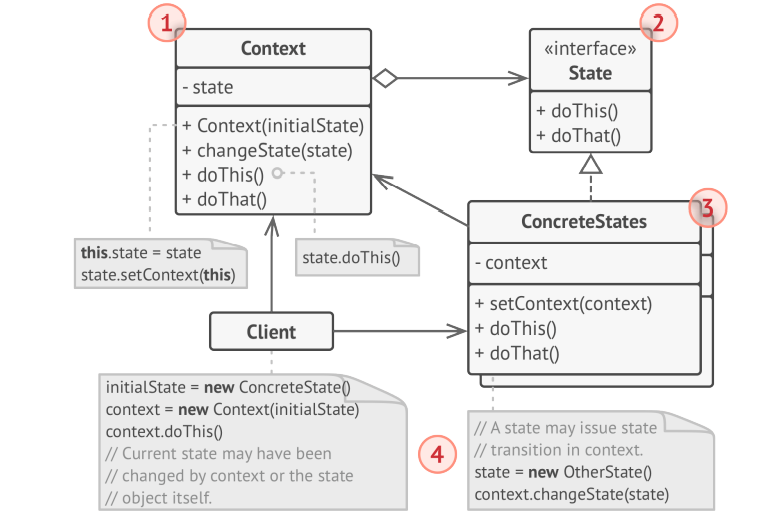
\includegraphics[scale=0.6]{image/behavioral/state.png}
\end{center}
\subsubsection{Ưu điểm và Nhược điểm}
Ta có rất nhiều ưu nhược điểm như sau:\\\\
Ưu điểm:
\begin{itemize}
    \item Mẫu State cho phép mô hình hóa trực quan các trạng thái khác nhau và cách chúng tương tác với nhau.
    \item Thay vì sử dụng nhiều câu lệnh điều kiện, mẫu State giúp tách biệt logic của từng trạng thái thành các lớp riêng biệt, giảm sự phức tạp của mã.
\end{itemize}
Nhược điểm:
\begin{itemize}
    \item Mẫu State có thể tạo ra nhiều lớp con để đại diện cho từng trạng thái, dẫn đến việc tăng số lượng lớp trong mã nguồn.
    \item Logic của mỗi trạng thái có thể phân mảnh trong các lớp con khác nhau, làm cho mã nguồn khó hiểu và duy trì.
\end{itemize}
\subsubsection{Code Example}
\begin{itemize}
    \item Có các class State con.
    \item Một các Context chữa State hiện tại.
\end{itemize}
\begin{lstlisting}
#include <iostream>

// State interface
class State {
public:
    virtual void handleState() = 0;
};

// Concrete states
class ConcreteStateA : public State {
public:
    void handleState() override {
        std::cout << "Handling state A." << std::endl;
    }
};

class ConcreteStateB : public State {
public:
    void handleState() override {
        std::cout << "Handling state B." << std::endl;
    }
};

// Context class
class Context {
private:
    State* currentState;

public:
    Context() {
        currentState = nullptr;
    }

    void setState(State* state) {
        currentState = state;
    }

    void request() {
        if (currentState) {
            currentState->handleState();
        }
    }
};

int main() {
    Context context;

    // Set initial state to A
    ConcreteStateA stateA;
    context.setState(&stateA);
    context.request();

    // Change state to B
    ConcreteStateB stateB;
    context.setState(&stateB);
    context.request();

    return 0;
}

\end{lstlisting}
Ở hàm main, Ta tạo 2 state r set State cho context r request nó sau đó chuyển context qua state khác rồi request nó.\\
\newline
\textbf{Kết quả:}
\begin{lstlisting}
Handling state A.
Handling state B.
\end{lstlisting}
\subsubsection{Các Pattern liên quan}
\begin{itemize}
    \item Bridge, State, Strategy có cấu trúc rất giống nhau. Tuy nhiên, chúng đều giải quyết các vấn đề khác nhau.
    \item State là bản mở rộng của Strategy. Cả hai Pattern đều dựa trên thành phần: chúng thay đổi hành vi của ngữ cảnh bằng cách ủy quyền một số công việc cho các object trợ giúp.
    \item Gần giống strategy, chuyển đổi các chiến lược thông qua các phương thức được định nghĩa trong interface. State không hạn chế sự phụ thuộc giữa các trạng thái cụ thể, cho phép chúng thay đổi trạng thái của ngữ cảnh theo ý muốn.
\end{itemize}


